% !TEX encoding = UTF-8 Unicode
\documentclass[a4paper]{article}

\usepackage{color}
\usepackage[obeyspaces]{url}
\usepackage[T1]{fontenc} % enable Cyrillic fonts
\usepackage[utf8]{inputenc} % make weird characters work
\usepackage{graphicx}
\usepackage[margin=1.0in]{geometry}
\usepackage[table]{xcolor}
\usepackage{tocloft}
\usepackage{float}
\addtolength{\cftsecnumwidth}{10pt}
\usepackage{wasysym}


\usepackage[english,serbian]{babel}
%\usepackage[english,serbianc]{babel} 

\PassOptionsToPackage{obeyspaces}{url}
\usepackage[unicode]{hyperref}
\hypersetup{colorlinks,citecolor=green,filecolor=green,linkcolor=blue,urlcolor=blue}

\usepackage{listings}
\renewcommand\lstlistingname{Kod}
\renewcommand\lstlistlistingname{Kodovi}

\definecolor{mygreen}{rgb}{0,0.6,0}
\definecolor{mygray}{rgb}{0.5,0.5,0.5}
\definecolor{mymauve}{rgb}{0.58,0,0.82}

\lstset{
  backgroundcolor=\color{white},   % choose the background color; you must add \usepackage{color} or \usepackage{xcolor}; should come as last argument
  basicstyle=\scriptsize\ttfamily,        % the size of the fonts that are used for the code
  breakatwhitespace=false,         % sets if automatic breaks should only happen at whitespace
  breaklines=true,                 % sets automatic line breaking
  captionpos=b,                    % sets the caption-position to bottom
  commentstyle=\color{mygreen},    % comment style
  deletekeywords={...},            % if you want to delete keywords from the given language
  escapeinside={\%*}{*)},          % if you want to add LaTeX within your code
  extendedchars=true,              % lets you use non-ASCII characters; for 8-bits encodings only, does not work with UTF-8
  firstnumber=1,                   % start line enumeration with line 1000
  frame=single,	                   % adds a frame around the code
  keepspaces=true,                 % keeps spaces in text, useful for keeping indentation of code (possibly needs columns=flexible)
  keywordstyle=\color{blue},       % keyword style
  language=Python,                 % the language of the code
  morekeywords={*,...},            % if you want to add more keywords to the set
  numbers=left,                    % where to put the line-numbers; possible values are (none, left, right)
  numbersep=5pt,                   % how far the line-numbers are from the code
  numberstyle=\tiny\color{mygray}, % the style that is used for the line-numbers
  rulecolor=\color{black},         % if not set, the frame-color may be changed on line-breaks within not-black text (e.g. comments (green here))
  showspaces=false,                % show spaces everywhere adding particular underscores; it overrides 'showstringspaces'
  showstringspaces=false,          % underline spaces within strings only
  showtabs=false,                  % show tabs within strings adding particular underscores
  stepnumber=2,                    % the step between two line-numbers. If it's 1, each line will be numbered
  stringstyle=\color{mymauve},     % string literal style
  tabsize=2,	                     % sets default tabsize to 2 spaces
  title=\lstname                   % show the filename of files included with \lstinputlisting; also try caption instead of title
}

\usepackage{enumitem}
\newlist{legal}{enumerate}{10}
\setlist[legal]{label*=\arabic*.}

\begin{document}

\title{Informacioni sistem pozorišta\\ \small{Seminarski rad u okviru kursa\\Informacioni sistemi\\ Matematički fakultet}}

\author{
Katarina Savičić 1086/2020\\
Dragana Milić 1042/2019\\
Nikola Vuković 1090/2020\\
Ognjen Milinković 1008/2020\\
Momir Adžemović 1005/2020
}

\date{1.~april 2020.}

\maketitle

\abstract

Ovo je sažetak.

\newpage

\tableofcontents

\newpage

\section{Uvod}
Ovaj rad se bavi modeliranjem najvažnijih procesa u radu jednog pozorišta, gde se akcenat
stavlja na proces produkcije predstave. Proces predstave se sastoji iz dva glavna 
dela:\cite{hamilton_theatre_producing_the_drama}
\begin{itemize}
  \item priprema i izvođenje
  \item tehnički deo
\end{itemize}

\section{Slučajevi upotrebe}

\subsection{Organizacija predstave}
\begin{enumerate}
  \item \textbf{Kratak opis:} Organizator predstave je zadužen za ceo proces formiranja predstave od njene prijave do realizacije. 
        Proces formiranja podrazumeva prijavu koju mora da odobri supervizor pozorišta, unajmljivanje 
        glumaca i rezervacija sala za predstave. Neophodno je da organizator konstantno ima uvid u stanje
        svake predstave za koji je on zadužen.
  \item \textbf{Učesnici:} \dots
  \item \textbf{Preduslovi:} \dots
  \item \textbf{Postuslovi:} \dots
  \item \textbf{Osnovni tok:} \dots
  \item \textbf{Alternativni tokovi:} \dots
  \item \textbf{Podtokovi:} \dots
  \item \textbf{Specijalni zahtevi:} \dots
  \item \textbf{Dodatne informacije:} \dots
% Adaptacija predstave (dramaturg)

% Ovo sve može u tok
% Da bi se predstava održala, potrebno je da organizator napravi predstavu u okviru IS-a. 
% Predstava ima inicijalno stanje \textit(prijava). Supervizor pozorišta može da odobri ili 
% odbije prijavljenu predstavu. Ako se prijavljena predstava odobri, onda predstava prelazi 
% u stanje \textit{odobrena}. Glumac može da se prijavi za jednu (ili više) uloga za predstavu koja je
% odobrena. Svaka odobrena predstava ima ulogu rezerva, za koju može da se prijavi bilo koji glumac. 
% Supervizor može da promeni stanje predstave koja ima stanje odobrena i ima popunjena mesta glumca 
% kao u pripremi. 
\end{enumerate}

\subsection{Rezervacija pozorišnih sala}
\begin{enumerate}
  \item \textbf{Kratak opis:} Organizator predstave u pripremi treba da rezerviše salu za probu, 
        audiciju ili konkretnu predstavu. Dakle, treba omogućiti uvid u slobodne sale, 
        kao i rezervacije unapred.
\end{enumerate}

\subsection{Audicije i konkursi za posao}
\begin{enumerate}
  \item \textbf{Kratak opis:} Konkursi mogu da podrazumevaju zapošljavanje za stalno ili privremeno
        (jedna ili više predstava). Konkursi mogu da se odnose na različite uloge kao što su
        organizator, glumac, itd... Audicije se odnose konkretno za glumce.
\end{enumerate}
 
\subsection{Prodaja karata}
Prodaja karata je proces koji sledi nakon što je određen datum, rezervisana sala i dodeljene uloge
zaposlenim. Tada je moguće odrediti preciznije budžet potreban za dalju realizaciju predstave, pa
samim tim i minimalni broj kupljenih karata za izvođenje. Na osnovu rezervisane sale (i potencijalno još 
nekih drugih faktora, kao što je epidemija ili slično), određuje se broj karata za prodaju. Budući
gledaoci predstave mogu da kupe ili rezervišu kartu za pozorište preko veb stranice pozorišta.

\subsubsection{Definisanje broja karata za predstavu}
\noindent\textbf{Kratak opis:} Organizator predstave može da definiše broj karata na osnovu rezervisane
sale za izvođenje predstave. Potrebno je da supervizor pozorišta odobri predstavu za izvođenje. 
Nakon odobrenja se ažurira repertoar na stranici pozorište.\\

\noindent\textbf{Učesnici:} Organizator predstave i supervizor pozorišta.\\

\noindent\textbf{Preduslovi:}
  \begin{itemize}
    \item Predstava je zakazana određenog datuma.
    \item Rezervisana je određena sala za predstavu.
    \item Dodeljene su sve uloge (tehničke i umetničke) za realizaciju predstave .
    \item Određen je potreban budžet za realizaciju.
    \item Organizator je zaduđen za barem jednu predstavu.
  \end{itemize}

\noindent\textbf{Postuslovi:} 
  \begin{itemize}
    \item Ažuriran je repertoar tj. dodata je nova predstava sa kratkim opisom i datumom izvođenja.
    \item Ažuriran je status predstave u bazi podataka.
    \item Korisnici su u mogućnosti da rezervišu ili kupe kartu za tu predstavu.
  \end{itemize}

\noindent\textbf{Osnovni tok:}
  \begin{legal}
    \item Organizator unosi podatke za prijavljivanje na sistem.
    \item Sistem vrši verifikaciju i prikazuje organizatoru listu predstava za koje je zadužen.
    \item Organizator bira predstavu koju želi da ažurira.
    \item Sistem prikazuje informacije o predstavi.
    \item Organizator unosi broj karata za prodaju i potencijalno dodaje napomenu.
    \item Sistem proverava unete podatke.
    \item Sistem ažurira bazu podataka.
  \end{legal}

\noindent\textbf{Alternativni tokovi:} 
\begin{itemize}
  \item \textbf{A1. Neuspelo prijavljivanje} 
      \begin{legal}
        \item Sistem prikazuje poruku o grešci pri prijavljivanju..
        \item Proces se nastavlja u \textbf{koraku 1}.
      \end{legal}
  \item \textbf{A2. Podaci o broju karata nisu validni} 
    \begin{legal}
      \item Sistem prikazuje poruku o grešci.
      \item Proces se nastavlja u \textbf{koraku 5}.
    \end{legal}
\end{itemize}

\noindent\textbf{Dodatne informacije:} Postoji period osvežavanja repertoara na stranici na osnovu
  sadržaja baze podataka.

\subsubsection{Registracija i prijavljivanje na stranicu pozorišta}

\subsubsection{Onlajn kupovina karata i rezervacija}

\textbf{Napomena:} Možda budem podelio na dva slučaja upotrebe (prethodni).\\

\noindent\textbf{Kratak opis:} Informacioni sistem nudi pregled repertoara korisnicima. 
        Svako može da kupi kartu za određenu predstavu ako postoji slobodno mesto.
        Alternativa je da se vrši rezervacija karte koja se kasnije može da kupi u blagajni.\\

\noindent\textbf{Učesnici:} Registrovan korisnik koji želi da kupi ili rezerviše kartu.\\

\noindent\textbf{Preduslovi:} 
  \begin{itemize}
    \item Korisnik mora da bude registrovan sa odgovarajućim mejlom. 
    \item Korisnik mora da ima pristup internetu.
    \item Sistem mora da bude u funkciji.
    \item Sistem mora da bude pouzdan. 
    \item Mora da postoji barem jedno slobodno mesto za željenu predstavu, a samim tim mora da 
          postoji barem jedna aktivna predstava. 
    \item Ukoliko korisnik želi da kupi kartu, mora da ima karticu za online plaćanje (ili 
          alternativu neku).
  \end{itemize}
  
\noindent\textbf{Postuslovi:} 
  \begin{itemize}
    \item Korisnik je dobio potvrdu na mejl sa kodom kupljenje ili rezervisane karte.
    \item Baza je ažurirana tj. broj karata za predstavu je umanjen za jedan.
  \end{itemize}

\noindent\textbf{Osnovni tok:}
  \begin{legal}
    \item Prijavljen korisnik pristupa stranici za kupovinu karata. 
    \item Sistem učitava podatke iz baze i prikazuje repertoar.
    \item Korisnik klikom bira željenu predstavu.
    \item Sistem otvara korisniku formu za rezervaciju ili kupovinu karte.
    \item Korisnik kupuje ili rezerviše kartu.
    \item Sistem proverava formu i ažurira bazu podataka.
    \item Sistem šalje mejl sa odgovarajućim kodom korisniku na mejl.
    \item Sistem prikazuje korisniku poruku o uspešnoj kupovili ili registraciji i podseća
          korisnika da proveri mejl.
  \end{legal}

\noindent\textbf{Alternativni tokovi:} 
  \begin{itemize}
    \item \textbf{A1. Korisnik nije prijavljen} 
        \begin{legal}
          \item Sistem otvara korisniku stranicu za prijavljivanje.
          \item Korisnik unosi odgovarajuće podatke i prijavljuje se.
          \item Sistem proverava da li se uneti podaci poklapaju sa podacima iz baze.
          \item Sistem započinje se sesiju korisnika (korisnik je prijavljen).
          \item Proces se nastavlja u \textbf{koraku 1}.
        \end{legal}
    \item \textbf{A2. Korisnik je već rezervisao kartu}
        \begin{legal}
          \item Sistem prikazuje korisniku obaveštenje o nemogućnosti rezervacije više od jedne karte.
          \item Korisnik pretiska dugme za potvrdu.
          \item Proces se nastavlja u \textbf{koraku 2}.
        \end{legal}
    \item \textbf{A3. Neuspešna kupovina karte}
        \begin{legal}
          \item Sistem prikazuje korisniku obaveštenje o neuspelom plaćanju sa odgovarajućim
                razlogom, ako je taj razlog poznat sistemu.
          \item Korisnik pretiska dugme za potvrdu.
          \item Proces se nastavlja u \textbf{koraku 5}.
        \end{legal}
    \item \textbf{A4. Tokom popunjavanja forme su rasprodate karte su se rasprodale}
        \begin{legal}
          \item Sistem prikazuje korisniku obaveštenje o rasprodatim kartama.
          \item Korisnik pretiska dugme za potvrdu.
          \item Proces se nastavlja u \textbf{koraku 2}.
        \end{legal}
  \end{itemize}

\noindent\textbf{Podtokovi:}
  \begin{itemize}
    \item \textbf{5.1. Kupovina karte}
        \begin{legal}
          \item Korisnik bira opciju za kupovinu karte.
          \item Korisnik Pretiska dugme za potvrdu.
          \item Sistem prikazuje korisniku opcije plaćanja.
          \item Korisnik bira željeni način plaćanja.
          \item Sistem prikazuje korisniku formu za plaćanje.
          \item Korisnik popunjava formu.
          \item Korisnik pretiska dugme za potvrdu.
          \item Sistem izvršava transakciju plaćanja sa odgovarajućim proveravama.
        \end{legal}
    \item \textbf{5.2. Rezervacija karte}
        \begin{legal}
          \item Korisnik bira opciju za rezervaciju karte.
          \item Korisnik pretiska dugme za potvrdu.
        \end{legal}
  \end{itemize}

\noindent\textbf{Specijalni zahtevi:} Mejl mora da stigne korisniku u roku od 5 minuta nakon što 
        je prikaza poruka o uspešnoj kupovini odnosno rezervaciji.\\

\noindent\textbf{Dodatne informacije:} Podaci koji su potrebni za prijavu su korisničko ime ili mejl, i 
        šifra naloga.

\begin{figure}[H]
  \begin{center}
      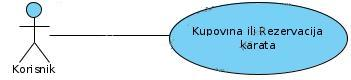
\includegraphics[width=50mm,height=20mm]{../diagrams/usecase_prodaja_karata.jpg}
  \end{center}
\end{figure}

\subsubsection{Kupovina karata uživo}
\noindent\textbf{Kratak opis:} Gledaoci koji su rezervisali kartu mogu da kupe kartu u pozorištu.
Gledaoci koji nisu rezervisali kartu u pozorišu mogu da kupe kartu ako i dalje postoji mesta.

\subsubsection{Zahtev za povraćaj novca}  
\noindent\textbf{Kratak opis:} Korisnik može da zahteva povraćaj nova pre ili posle izvođenja predstave.

\subsubsection{Povraćaj novca za otkazanu predstavu}
\noindent\textbf{Kratak opis:} Ukoliko organizator ili supervizor otkažu predstavu, potrebno je
da se vrati novac korisnicima koji su kupili kartu. Takođe je potrebno da se svim korisnicima koji
su rezervisali kartu, pošalje mejl kao obaveštenje o otkazivanju predstave.

\subsection{Vođenje finansija}
\begin{enumerate}
  \item \textbf{Kratak opis:} Supervizor pozorišta može da vidi prilive i odlive za ceo sistem ili
        neku konkretnu predstavu. 
\end{enumerate}

\section{Druga sekcija.}
Ovo je druga sekcija.

\section{Treća sekcija.}
Ovo je treća sekcija.

\section{Zaključak}
Ovo je zaključak.

\newpage

\addcontentsline{toc}{section}{Literatura}
\appendix
\bibliography{literatura} 
\bibliographystyle{unsrt}

\end{document}
        